\section{Theorie}
Ein Laser besteht grundlegend aus drei Komponenten.
Einem aktiven Medium, einer Pumpquelle und einem Resonator.
Im Generellen wird versucht, das Lasermedium zu manipulieren,
sodass das einfallende Licht verstärkt wird.
Dies passiert durch Wechselwirkung des Strahlenfeldes mit dem Lasermaterial.
Es gibt drei Möglichkeiten, wie Photonen in Wechselwirkungsprozessen auftreten können.
Grafisch dargestellt ist dies in Abbildung \ref{fig:emission}.

\begin{figure}[H]
  \centering
  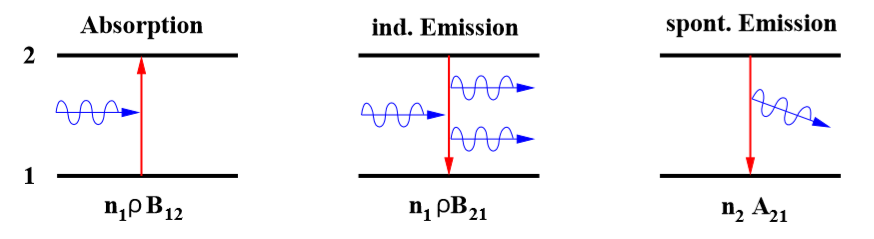
\includegraphics[width=0.9\textwidth]{Bilder/emission.png}
  \caption{Schematische Darstellung von Absorption und Emission eines Photons.\cite{anleitung}}
  \label{fig:emission}
\end{figure}

Das einfallende Photon kann absorbiert werden, wenn die Energie dessen gleich der Energie des Übergangs zwischen den Energieniveaus ist.
Für eine Emission gibt es zwei Varianten.
Es ist zum einen möglich, dass eine Emission induziert wird, wenn ein externes Photon eintrifft.
Hierbei geht ein Atom aufgrund dessen vom angeregten Zustand in den Grundzustand unter Aussendung eines Photons über.
Das eintreffende und das ausgehende Photon stimmt hierbei in Energie, Phase und Ausbreitungsrichtung überein.
Dieser Vorgang der Photonemission kann aber auch spontan passieren.
Der Zusammenhang zwischen der Anzahl der Photonen, die pro Volumeneinheit pro Sekunde induziert emittiert werden wird durch den Zusammenhang
\begin{equation}
  \dot{N} = n_2\rho(\nu)B_\text{21}
\end{equation}
beschrieben.
Hierbei sind $n$ der besetzte Zustand, $\rho$ die Energiedichte des Strahlungsfeldes und $B_\text{21}$ der Einsteinkoeffizient als Maß für die Übergangswahrscheinlichkeit von einem Zustand zum anderen.
Durch die Betrachtung im thermischen Gleichgewicht folgt nach der Boltzmann-Statistik, dass die Besetzung des Grundzustandes dominiert.
Um die für die Funktionsweise des Lasers geforderte Kohärenz und somit eine Verstärkung des einfallenden Lichts zu erhalten, ist es nötig, dass die induzierte gegenüber der spontanen Emission überwiegt.
Nötig ist hierfür eine Besetzungsinversion.
Dadurch wird eine höhere Besetzung des angeregten als des Grundzustandes verstanden.
Um dies für das Experiment zu erreichen wird dem Lasermedium konstant Energie von Außen hinzugefügt.
Dies wird als Pumpen bezeichnet.
Als Resonator wird die Laufstrecke des Laserstrahls ausgehend vom Lasermedium zwischen den beiden reflektierenden Spiegeln an den Resonatorenden verstanden, wie Abbildung \ref{fig:resonator} zeigt.
Damit der Laserstrahl einen möglichst langen Laufweg hat, sind eben diese Spiegel installiert, da die Verstärkung exponentiell mit der Laufweglänge im aktiven Medium wächst.

\begin{figure}[H]
  \centering
  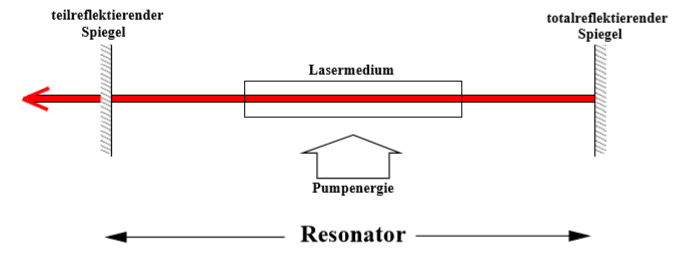
\includegraphics[width=0.9\textwidth]{Bilder/resonator.png}
  \caption{Schematischer Aufbau eines Lasers mit seinen drei Grundkomponenten.\cite{anleitung}}
  \label{fig:resonator}
\end{figure}

Einer der Spiegel ist teildurchlässig, damit der Laserstrahl zu einer Seite hin ausgekoppelt werden kann.
Die Spiegel des optischen Resonators können aus zwei planparallelen, zwei sphärischen oder aus einer Kombination bestehen.
Damit es zu Oszillatorverhalten kommt, müssen die Verluste durch die Spiegel möglichst gering gehalten werden.
Sobald die Resonatorverluste kleiner als die Verstärkung durch die induzierte Emission ist, ist ein selbsterregender Resonator gegeben.
Somit gilt für einen stabilen Resonator
\begin{equation}
  0 \leq g_1 \cdot g_2 \leq 1.
\end{equation}
Die Resonatorparameter sind im Allgemeinen gegeben durch $g_i=1-L/r_i$ gegeben;
die Krümmungsradien $r_i$ der Spiegel und die Resonatorlänge $L$ sind hierbei veränderlich.
